\documentclass{article}

\usepackage{url} 

\usepackage{pdfpages}
\usepackage{lastpage}
\usepackage{fancyhdr}
\usepackage{ngerman}
\usepackage{listings}

\usepackage{floatrow}
\usepackage[tableposition=top]{caption}
\floatsetup[table]{capposition=top}

\usepackage{amsmath, amssymb}

\usepackage[utf8]{inputenc}


\usepackage[numbib]{tocbibind}



\newcommand\twodigits[1]{%
   \ifnum#1<10 0#1\else #1\fi
}



\lhead{Transformator}
\rhead{23. Oktober 2020\\T. Maier, J. Winkler}
%\cfoot{\twodigits{\thepage}~/ \pageref{LastPage}}
\cfoot{{\thepage}~/ \pageref{LastPage}}

\newcommand{\W}{\text{W}}
\newcommand{\V}{\text{V}}
\newcommand{\A}{\text{A}}





\begin{document}

\parindent0cm

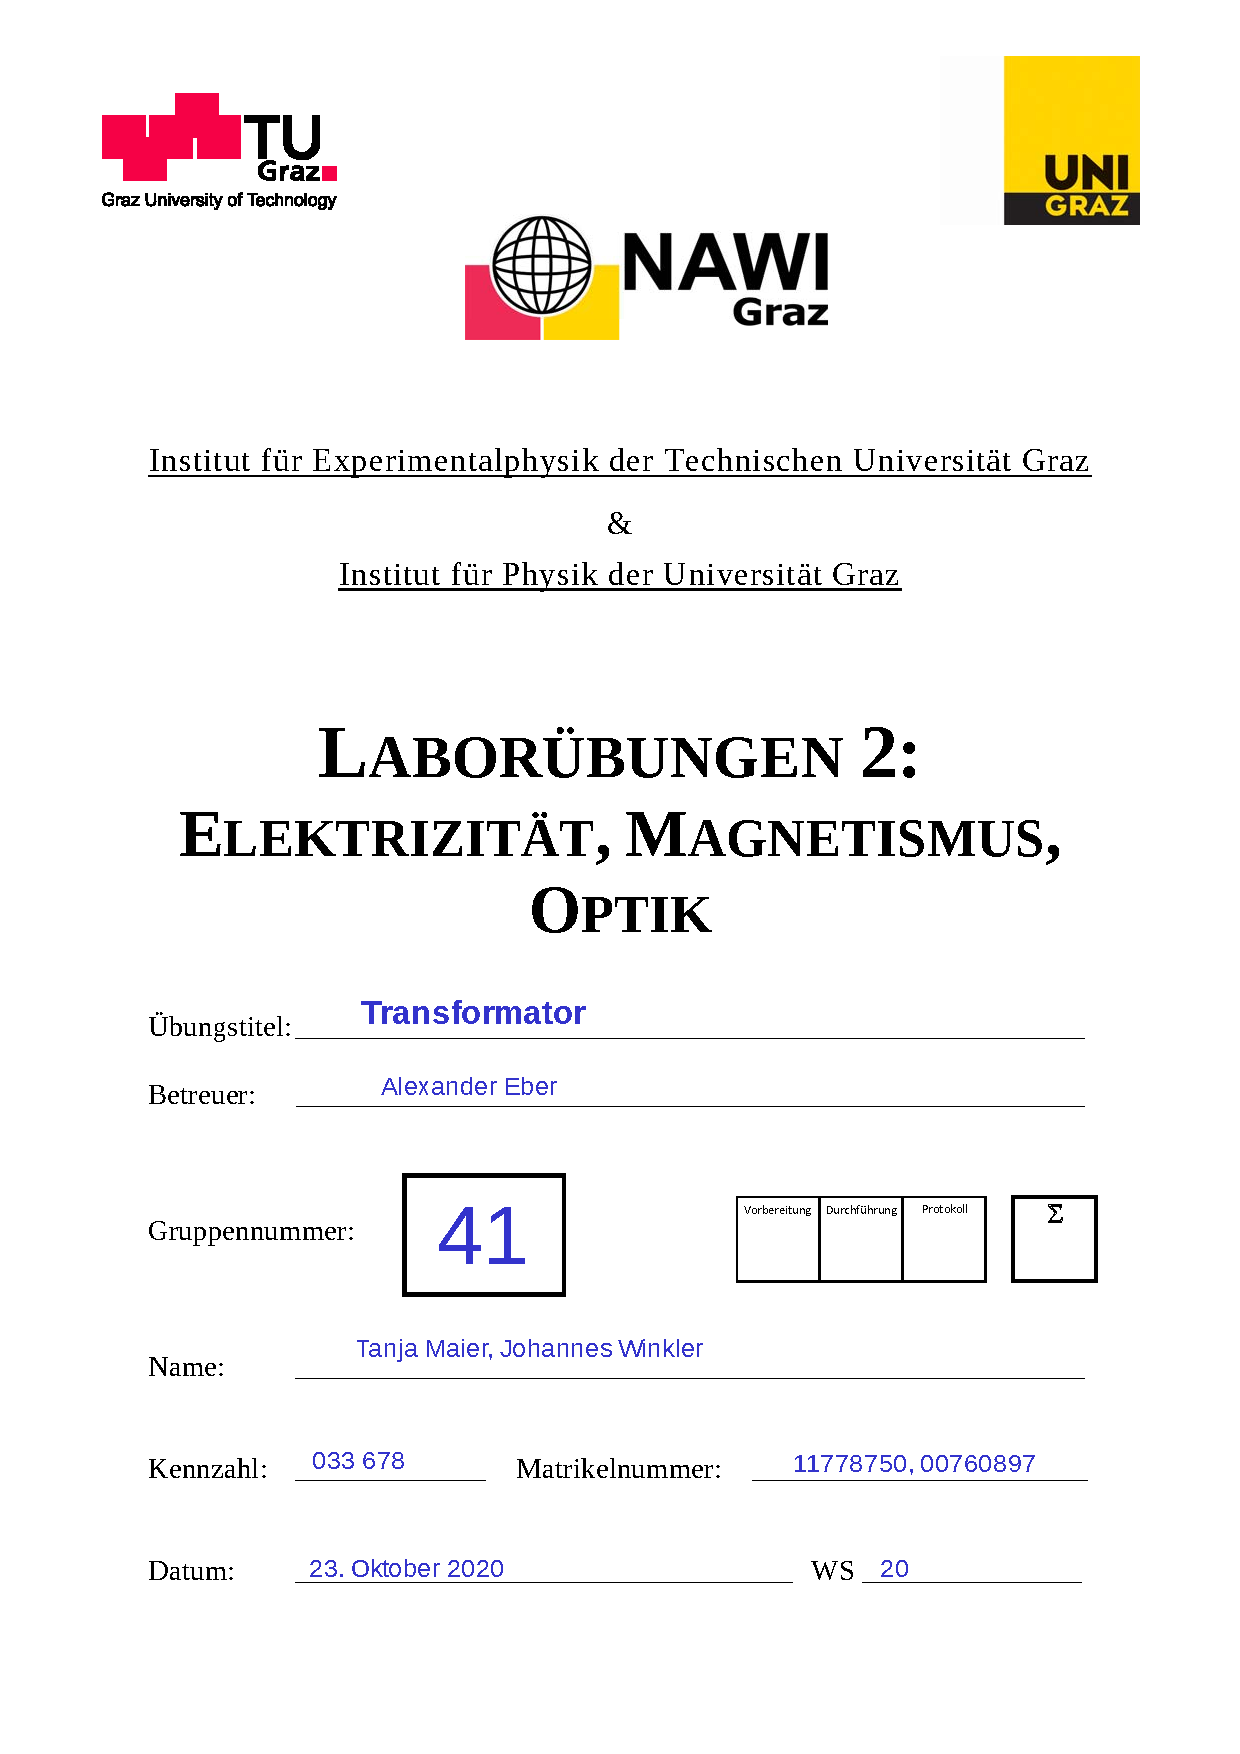
\includepdf{Deckblatt.pdf}


\pagestyle{fancy}

\section{Aufgabenstellung}

\begin{enumerate}
\item Messen von Primärstrom, Primärspannung, Wirkleistung und Sekundärspannung im Leerlauf sowie Durchführung der Berechnungen von Scheinleistung primär, Leistungsfaktor, Verlustleistung, Blindleistung primär, Wirkleistung sekundär und Wirkungsgrad. Oszillographische Darstellung von Primärstrom und Sekundärspannung.
\item Messen von Primärstrom, Primärspannung, Wirkleistung und Sekundärspannung mit sekundärseitiger Ohm’scher Last sowie Durchführung der Berechnungen von Scheinleistung primär, Leistungsfaktor, Verlustleistung, Blindleistung primär, Wirkleistung sekundär und Wirkungsgrad. Oszillographische Darstellung von Primärstrom und Sekundärspannung.
\item Messen von Primärstrom, Primärspannung, Wirkleistung und Sekundärspannung mit Ohm'scher induktiver Last sowie Erstellung eines Diagramms von Leistung über Lastwiderstand. Oszillographische Darstellung von Primärstrom und Sekundärspannung.
\end{enumerate}



\section{Grundlagen und Versuchsaufbau}




\begin{figure}[H]
\caption{Versuchsaufbau Transformator. Tr1 Regeltrenntrafo, Tr2 Messtrafo, $R_s$ Shunt ($0.5~\Omega$), $I_1$ Primärstrom, $I_2$ Sekundärstrom, $U_1$ Primärspannung, $U_2$ Sekundärspannung, $N_{1W}$ Leistungsmessung}
\label{fig:pic1}
{\centering
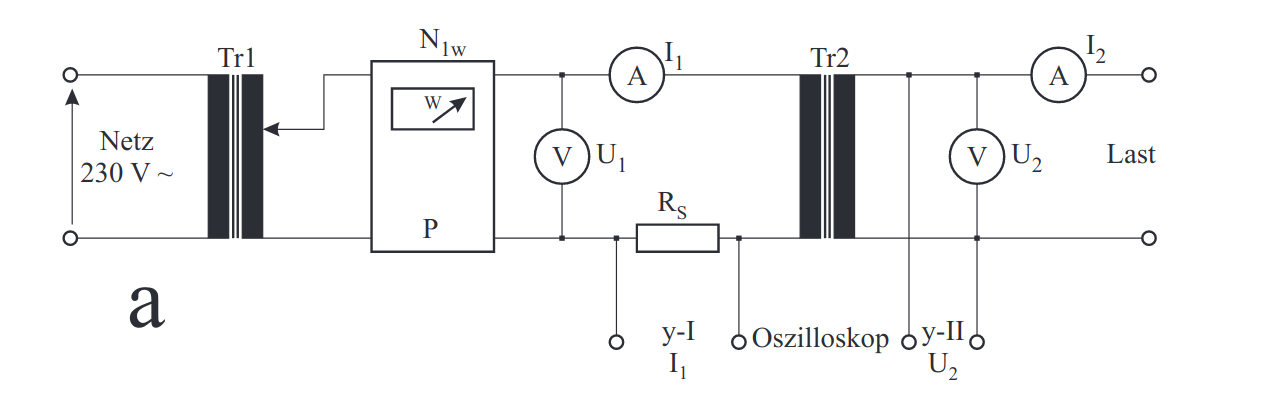
\includegraphics[scale=0.9]{pic1.png}
~
}
\end{figure}



\section{Geräteliste}

\begin{table}[H]
\caption{Liste der verwendeten Geräte}

~

\begin{tabular}{l|llll}
Kürzel & Bezeichnung & Hersteller & Gerätenummer & Unsicherheit \\
\hline
DM & Digitalmultimeter & Leybold \\
TF & Transformator & Ruhstrat \\
A1 & Amperemeter 1 & Norma & & $\pm 1.5\%$ \\
A2 & Amperemeter 2 & Norma & & $\pm 1.5\%$ \\
V1 & Voltmeter 1 & Norma & & $\pm 0.5\%$ \\
V2 & Voltmeter 2 & Norma & VII/1121/3 & $\pm 0.5\%$ \\
SP & Spule \\
WS & Widerstand  & & VII/695 \\
LWS & Lastwiderstand \\
OS & Oszilloskop & Rigol \\
TT & Trenntrafo & Ruhstrat 
\end{tabular}

\end{table}




\section{Durchführung und Messwerte}

\subsection{Leerlauf}

Zuerst wurde die Schaltung gemäß Abbildung \ref{fig:pic1} aufgebaut, jedoch ohne das Amperemeter für den Sekundärstrom. Dan wurde eine Primärspannung von $U_1= 160~$V angelegt. Die Unsicherheit bei Voltmetern sind $0.5\%$, bei Amperemetern $1.5\%$. Daher gilt insgesamt 
\begin{align*}
U_1 &= (160 \pm 1)~\V \\
U_2 &= (17.6 \pm 0.1)~\V \\
I_1 &= (0.20 \pm 0.01)~\A \\
P_1 &= (6.9 \pm 0.1)~\W
\end{align*}
Da der Transformator im Leerlauf war, ist $I_2 = 0$ zu setzen.


\subsection{Ohm'sche Last}

Hier wird derselbe Aufbau verwendet, jedoch zusätzlich mit einem Verbraucher an der Sekundärseite. Es wird hier zusätzlich zur Sekundärspannung auch der Sekundärstrom $I_2$ gemessen. Der variable Widerstand wurde so gewählt, dass $I_2 < 1~\A$ ist. Es gilt
\begin{align*}
U_1 &= (160 \pm 1)~\V \\
U_2 &= (16.6 \pm 0.1)~\V \\
I_1 &= (0.24 \pm 0.01)~\A \\
I_2 &= (0.68 \pm 0.02)~\A \\
P_1 &= (19.3\pm0.1)~\W
\end{align*}





\subsection{Ohm + Induktive Last}

Zum vorherigen Aufbau wurde eine Spule $(L=0.1~$H) sekundärseitig in Serie geschalten. Für die übliche Primärspannung $U_1 = (160\pm1.2)~\V$ wurden 15 Messwerte bei unterschiedlicher Einstellung des Lastenwiderstandes (bis zu 45~$\Omega$) gemessen. 

Es wird der Sekundärstrom $I_2$ und die Sekundärspannung $U_2$ gemessen, der variable Widerstand $R$ ergibt sich daraus. Die Leistung kann dadurch direkt berechnet weren. Die Messwerte sind in Tabelle \ref{tab:spule} zu finden.

\begin{table}[H]
\centering
\caption{Messwerte für Sekundärspannung $U_2$, Sekundärstrom $I_2$, Widerstand $R$}
\label{tab:spule}
\begin{tabular}{r|rrr}
  &	$U_2$ / V  &	$I_2$ /A  &	$R / \Omega$\\
  \hline
1 &	2.2	&0.53	&	4.2	 \\
2 &	2.7	&0.51	&	5.3	 \\
3 &	3.4	&0.49	&	6.9   \\
4 &	3.9	&0.46	&	8.5	  \\
5 &	4.2	&0.45	&	9.3	  \\
6 &	4.8	&0.43	&	11.2	  \\
7 &	5.3	&0.40	&   13.3  \\
8 &	5.9	&0.37	&	15.9	 \\
9 &	6.5	&0.32	&	20.3	 \\
10&	6.9	&0.29	&	23.8	 \\
11&	7.1	&0.27	&	26.3	  \\
12&	7.3	&0.25	&	29.2	  \\
13&	7.5	&0.23	&	32.6	 \\
14&	7.6	&0.21	&	36.2  \\
15&	7.7	&0.2		&   38.5 
\end{tabular}

\end{table}




\section{Auswertung}

\subsection{Leerlauf}
Für die Scheinleistung auf der Primärseite ergibt sich
\begin{align*}
S_1 = U_1\cdot I_1 = 32~\text{W}
\end{align*}
Die Fehlerrechnung ergibt
\begin{align*}
\Delta S_1 &= \Delta U_1\cdot I_1 + U_1\cdot \Delta I_1 = 1.68~\W \approx 2~\W
\end{align*}

Die Blindleistung ist
\begin{align*}
Q_1 = \sqrt{S_1^2 - P_1^2} = 31.25~\W
\end{align*}
Für die Fehlerrechnung gilt
\begin{align*}
\Delta Q_1 = \frac{S_1\cdot \Delta S_1}{\sqrt{S_1^2-P_1^2}} + \frac{P_1\cdot \Delta P_1}{\sqrt{S_1^2-P_1^2}} \approx 1.75~\W \approx 2~\W
\end{align*}

Der Leistungsfaktor ist
\begin{align*}
\cos(\phi) = \frac{P_1}{S_1} = 0.22
\end{align*}
Für die Fehlerrechnung gilt
\begin{align*}
\Delta\cos(\phi) = \frac{\Delta P_1}{S_1} + \frac{P_1}{S_1^2}\cdot \Delta S_1 = 0.01
\end{align*}

\subsection{Ohm'sche Last}

Analog zum Leerlauf gilt hier für die Scheinleistung
\begin{align*}
S_1 &= 37.6~\W \\
\Delta S_1 &= 1.7~\W
\end{align*}
Die Blindleistung ergibt
\begin{align*}
Q_1 &= 37~\W \\
\Delta Q_1 &= 2~\W
\end{align*}
Der Leistungsfaktor ist
\begin{align*}
\cos(\phi) &= 0.18 \\
\Delta \cos(\phi) &= 0.01
\end{align*}

Zusätzlich kann man jetzt die Sekundärseitige Wirkleistung berechnen (unter Annahme der Ohm'schen Last)
\begin{align*}
P_2 = U_2\cdot I_2 = 11.3~\text{W}
\end{align*}
Die Fehlerrechnung ergibt
\begin{align*}
\Delta P_2 &= \Delta U_2\cdot I_2 + U_2\cdot \Delta I_2 = 0.4~\W
\end{align*}


Der Wirkungsgrad kann folgend berechnet werden
\begin{align*}
\eta &= \frac{P_2}{P_1} = 0.58 \\
\Delta \eta &= \frac{\Delta P_2}{P_1} + \frac{P_2}{P_1^2}\cdot \Delta P_2 = 0.02
\end{align*}

Es fehlt noch die Verlustleistung und die dazugehörige Fehlerrechnung
\begin{align*}
P_V &= P_1-P_2 = 8.0~\W\\
\Delta P_V &= \Delta P_1 + \Delta P_2 = 0.5~\W
\end{align*}


\subsection{Ohm + Induktive Last}

An dieser Stelle wird die Leistung auf der Sekundärseite ausgewertet. Das Maximum befindet sich bei $U_2=5.9~\V$ und $I_2=0.37~\A$. Die maximale Leistung ist dann $P_2=2.18~\W$.

\begin{table}[H]
\centering
\caption{Berechnung der Leistung $P_2$ aus Sekundärspannung $U_2$, Sekundärstrom $I_2$ und bestimmung des Maximums.}
\label{tab:spule}
\begin{tabular}{r|rrrr}
  &	$U_2$ / V  &	$I_2$ /A  &	$R / \Omega$ & $P_2$ / W \\
  \hline
1 &	2.2	&0.53	&	4.2	 &	1.17 \\
2 &	2.7	&0.51	&	5.3	 &	1.38 \\
3 &	3.4	&0.49	&	6.9  &	1.67 \\
4 &	3.9	&0.46	&	8.5	 &	1.79 \\
5 &	4.2	&0.45	&	9.3	 &	1.89 \\
6 &	4.8	&0.43	&	11.2	 &	2.06 \\
7 &	5.3	&0.4		&   13.3 &	2.12 \\
{\color{red}8} &	\color{red} 5.9	& \color{red} 0.37	& \color{red} 15.9	 &	\color{red} 2.18 \\
9 &	6.5	&0.32	&	20.3	 &	2.08 \\
10&	6.9	&0.29	&	23.8	 &	2.00 \\
11&	7.1	&0.27	&	26.3	 &	1.92 \\
12&	7.3	&0.25	&	29.2	 &	1.83 \\
13&	7.5	&0.23	&	32.6	 & 	1.73 \\
14&	7.6	&0.21	&	36.2 &	1.60 \\
15&	7.7	&0.2		&   38.5 &	1.54
\end{tabular}

\end{table}

\section{Zusammenfassung}

Für den Leerlauf gilt
\begin{align*}
S_1 &= (32 \pm 2)~\W \\
Q_1 &= (31 \pm 2)~\W \\
\cos(\phi) &= (0.22 \pm 0.01)
\end{align*}
Da $I_2=0$ ist, gilt natürlich auch $P_2=0$ und $\eta = 0$.


Für die Ohm'sche Last gilt
\begin{align*}
S_1 &= (38 \pm 2)~\W \\
Q_1 &= (37 \pm 2)~\W \\
\cos(\phi) &= (0.18 \pm 0.01) \\
P_2 &= (11.3 \pm 0.4)~\W \\
\eta &= (0.58 \pm 0.02) \\
P_V &= (8.0 \pm 0.5)~\W
\end{align*}


Für die Ohm'sche Last mit in Serie geschalteter Spule ergibt sich ein Leistungsmaximum von $2.18~\W$ bei $R=15.9~\Omega$.

\section{Diskussion}



\begin{figure}[H]
\caption{Transformator im Leerlauf. Channel 1 ist proportional zum Primärstrom, Channel 2 ist Sekundärspannung}
\label{fig:task1}
{\centering
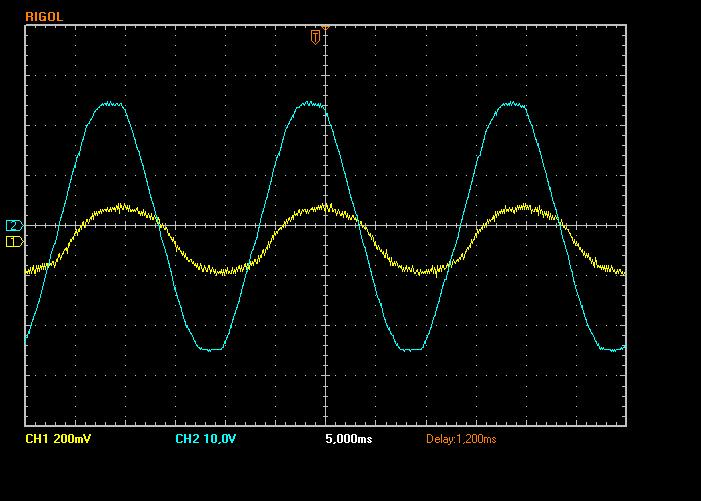
\includegraphics[scale=0.4]{task1.jpg}
~
}
\end{figure}

\begin{figure}[H]
\caption{Transformator mit Leerlauf. Channel 1 ist proportional zum Primärstrom, Channel 2 ist Sekundärspannung}
\label{fig:task1}
{\centering
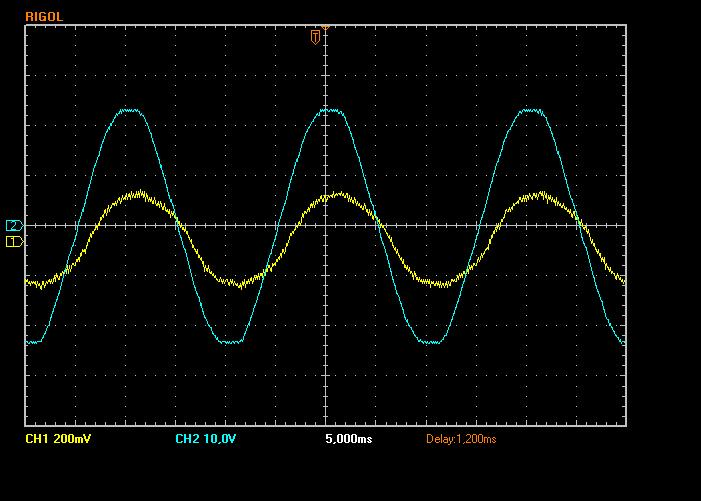
\includegraphics[scale=0.4]{task2.jpg}
~
}
\end{figure}

\begin{figure}[H]
\caption{Transformator mit mit ohm'scher und induktiver Belastung. Leistung und Widerstand als Kurve dargestellt.}
\label{fig:task1}
{\centering
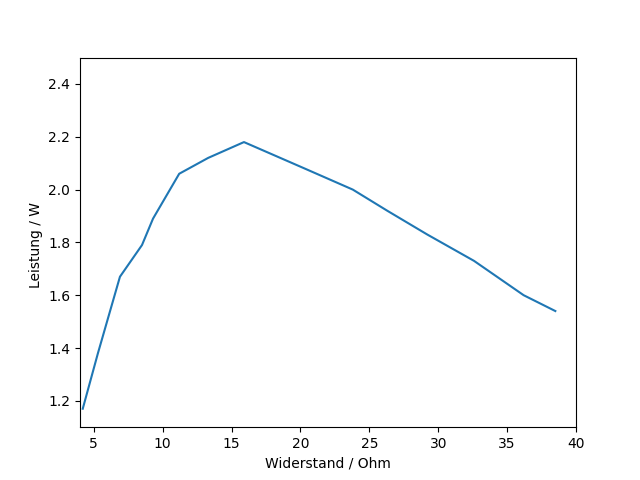
\includegraphics[scale=0.7]{kurve.png}
~
}
\end{figure}






%\newpage 
\appendix
\section{Python Skript}



\definecolor{commentgreen}{RGB}{2,112,10}
\definecolor{eminence}{RGB}{108,48,130}
\definecolor{weborange}{RGB}{255,165,0}
\definecolor{frenchplum}{RGB}{129,20,83}

\lstdefinelanguage{python}{
    morekeywords={def, for, range, abs, return},
    otherkeywords={<-,->, |>, \%\{, \}, \{, \, (, )},
    sensitive=true,
    morecomment=[l]{\#},
    morecomment=[n]{/*}{*/},
    morecomment=[s][\color{purple}]{:}{\ },
    morestring=[s][\color{orange}]"",
    commentstyle=\color{commentgreen},
    keywordstyle=\color{eminence},
    stringstyle=\color{red},
	basicstyle=\ttfamily,
	breaklines,
	showstringspaces=false,
	frame=tb
}
\lstinputlisting[language=Python,captionpos=b, label=lst:test,caption={Python Skript}]{generate_numbers.py}

%\lstinputlisting[language=Python,captionpos=b, label=lst:test,caption={Bessel Auswertung}]{generate_numbers_bessel.py}


%\lstinputlisting[language=Python,captionpos=b, label=lst:test,caption={Zerstreuungslinse Auswertung}]{generate_numbers_zerstreuungslinse.py}


\begin{thebibliography}{9}
\bibitem{chemie} \url{https://www.chemie.de/lexikon/Elektrochemisches_äquivalent.html}, 22.10.2020 22:53 Uhr
\bibitem{tu} bereitgestellte Unterlagen zum Versuch aus dem TeachCenter der TU Graz
\end{thebibliography}


\end{document}
